\documentclass[12pt,fleqn]{article}\usepackage{../common}
\begin{document}


$$ 
c = \frac{ 2c_m}{1 + \cosh |b_c(t-t_{mc})|   }
$$


\begin{minted}[fontsize=\footnotesize]{python}
from scipy.optimize import fmin
import pandas as pd
df = pd.read_csv('us.csv',sep='\s')
#df = pd.read_csv('oil1.csv',sep='\s')
df = df[df['year'] < 1966]
#df = df[df['year'] < 2008]

def hubbard_err(w):
    cm=w[0];bc=w[1];tmc=w[2]
    yfit = 2*cm / (1+cosh(bc*(df['year']-tmc)))
    diff = df['oil']-yfit
    e=norm(diff)
    return e

v = fmin(hubbard_err, [3, 3, 2000], maxiter=100000, maxfun=10000)
print v
\end{minted}

\begin{verbatim}
Optimization terminated successfully.
         Current function value: 12120221.612167
         Iterations: 86
         Function evaluations: 172
[  7.02607678e+00  -7.54324342e-04   1.96427493e+03]
\end{verbatim}

\begin{minted}[fontsize=\footnotesize]{python}
df2 = df.set_index('year')
ax = df2['oil'].plot(title='World Oil Production')
ax.set_ylabel("Barrels (Million)")
plt.savefig('peak_01.png')
\end{minted}


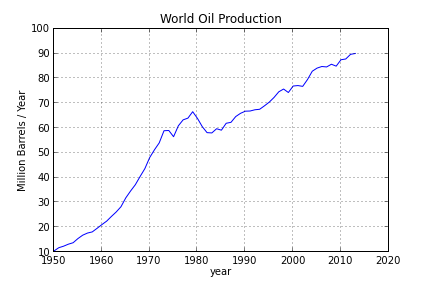
\includegraphics[height=6cm]{peak_01.png}

\begin{minted}[fontsize=\footnotesize]{python}
cm=v[0];bc=v[1];tmc=v[2]
def hubbard(x): 
    return 2*cm / (1+cosh(bc*(x-tmc)))
pred = map(hubbard, df['year'])
print pred
\end{minted}

\begin{verbatim}
[18.519947897246944, 19.314578111406714, 20.138017590457544, 20.990818356218071, 21.873493835070867, 22.786512989161988, 23.730294065627863, 24.705197966238885, 25.711521244217437, 26.749488739965617, 27.819245873049223, 28.920850614047456, 30.054265166797538, 31.219347399136325, 32.415842068444974, 33.643371897100387, 34.901428562271072, 36.189363674283257, 37.506379827920988, 38.851521821377311, 40.223668147980938, 41.621522876089223, 43.043608042442393, 44.488256693557283, 45.953606718119573, 47.437595620498556, 48.93795639112443, 50.452214633183004, 51.977687106537616, 53.511481848619326, 55.050500027886962, 56.591439678018837, 58.130801449970193, 59.664896504177811, 61.189856646347891, 62.701646787342689, 64.196079780704423, 65.668833660453231, 67.115471267231669, 68.531462213036434, 69.912207094218473, 71.253063819823694, 72.549375878505785, 73.796502323110687, 74.989849208656523, 76.124902177944563, 77.197259850616845, 78.202667637321611, 79.137051571929504, 79.996551732563404, 80.777554807551127, 81.476725356107835, 82.091035316239356, 82.617791324414171, 83.054659433116882, 83.399686843309581, 83.651320308649588, 83.808420916304343, 83.870275004363705, 83.836601036927561, 83.707552323482901, 83.483715537571612, 83.166105059272297, 82.756153234920987]
\end{verbatim}

\begin{minted}[fontsize=\footnotesize]{python}
df2['pred'] = pred
ax = df2['oil'].plot(title='World Oil Production')
ax.set_ylabel("Barrels (Million)")
ax.hold(True)
ax = df2['pred'].plot()
plt.savefig('peak_02.png')
\end{minted}

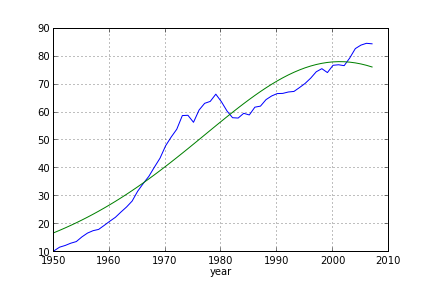
\includegraphics[height=6cm]{peak_02.png}


\url{http://www.earth-policy.org/Updates/2007/Update67_data2.htm#table1}

\url{http://en.wikipedia.org/wiki/Hubbert_curve}

\url{http://www.eia.gov/cfapps/ipdbproject/iedindex3.cfm?tid=5&pid=53&aid=1&cid=ww,&syid=1980&eyid=2013&unit=TBPD}

\url{http://www.countercurrents.org/mushalik270314.htm}

\url{http://www.eia.gov/dnav/pet/hist/LeafHandler.ashx?n=PET&s=MCRFPUS1&f=A}

\end{document}
